\documentclass[12pt,letterpaper]{article}

\usepackage{graphicx,
			amssymb,
			amsmath,
			titlesec,
			lipsum,
			setspace,
			lastpage,
			fancyhdr,
			tikz,
			titling}
\usepackage{tkz-euclide}
\usepackage{setspace}
\usepackage{hyperref}

\usetkzobj{all}
\usetikzlibrary{shapes,arrows}
\tikzstyle{block} = [rectangle, draw, fill=blue!20,
text centered, rounded corners, minimum height=2em]

\tikzstyle{line} = [draw, -latex']
\newenvironment{my_enumerate}{
	\begin{enumerate}
	\setlength{\itemsep}{1pt}
	\setlength{\parskip}{0pt}
	\setlength{\parsep}{0pt}}{\end{enumerate}
}

%% Figure caption formatting
\usepackage[labelfont=it,textfont=it,labelsep=period]{caption}
\usepackage[labelfont=it,textfont=it,labelsep=period]{subcaption}

%% Overall margins
\usepackage[margin=1in]{geometry}

%% Footer formatting
\fancyhf{}
\renewcommand{\headrulewidth}{0pt}
\pagestyle{fancy}
\cfoot{\textbf{\textsf{Page\ \thepage\ of \pageref{LastPage}}}}

%% Author list formatting
\newenvironment{nscenter}
 {\parskip=0pt\par\nopagebreak\centering}
 {\par\noindent\ignorespacesafterend}

\newcommand{\affiliatedauthor}[2]{
\begin{nscenter}
	#1 \\ \textit{#2}
\end{nscenter}
}

%% Abstract formatting
\renewcommand{\abstractname}{ABSTRACT}

\renewenvironment{abstract}
 {\vspace{-0.5ex}
	\small
	\begin{center}
		\bfseries \abstractname\vspace{-4ex}\vspace{0pt}
	\end{center}
	\list{}{
		\setlength{\leftmargin}{0.5in}
		\setlength{\rightmargin}{\leftmargin}
	}
	\item\relax}
 {\endlist}

%% Section header formatting
\renewcommand\thesection{}
\renewcommand\thesubsection{}
\renewcommand\thesubsubsection{}
\titleformat{\section}{\normalfont\bfseries}{\thesection}{1em}{}
\titleformat{\subsection}{\normalfont\bfseries}{\thesubsection}{1em}{}
\titleformat{\subsubsection}{\normalfont\itshape}{\thesubsubsection}{1em}{}
\titlespacing*{\section}{0pt}{2ex}{-1.5ex}
\titlespacing*{\subsection}{0pt}{2ex}{-1.5ex}
\titlespacing*{\subsubsection}{0pt}{2ex}{-1.5ex}

%% Paragraph formatting (changing this messes with literally everything)
\setlength{\parindent}{0pt}
\setlength{\parskip}{2ex}
\newcommand\tab[1][1cm]{\hspace*{#1}}

\title{Intelligent Quadcopter for IARC 2019}

\begin{document}

\begin{center}
	\textbf{\LARGE{\thetitle}}
\end{center}

%%%%%%%%%%%% SET AUTHOR NAMES AND AFFILIATIONS %%%%%%%%%%%%
\affiliatedauthor{Umer Salman, Noel Brownback, Eric Johnson, Mario Gonzalez}{The University of Texas at Austin}
%%%%%%%%%%%%%%%%%%%%%%%%%%%%%%%%%%%%%%%%%%%%%%%%%%%%%%%%%%%


%%%%%%%%%%%%%%%%%%%%%%% ABSTRACT %%%%%%%%%%%%%%%%%%%%%%%
\begin{abstract}
	Texas Aerial Robotics has constructed a custom quadrotor aircraft system for the fulfillment of the International Aerial Robotics Competition Mission 8. A combination of lightweight materials and powerful propulsion optimizes flight time, while standardized flight control systems supported by a massive community enables customization and adaptation to the mission at hand. This includes the integration of a multitude of sensors that enhance environmental awareness and allow for the aiding of people to analyze and interact with an environment. This is done through homebrewed QR code decoding algorithms and the shared computing power onboard the multiple aircrafts. Safe development has been assured by strategic selection of components, thorough vetting of software in Software in the Loop simulation, and robust testing procedures in secure areas.
\end{abstract}
%%%%%%%%%%%%%%%%%%%%%%%%%%%%%%%%%%%%%%%%%%%%%%%%%%%%%%%%

%%%%%%%%%%%%%%%%%%%%%% MAIN TEXT %%%%%%%%%%%%%%%%%%%%%%

\section*{INTRODUCTION}
	Previous aerial robotics missions have always allowed for GPS or set navigation points that allowed for constant locational awareness for the drone. Location data is important to any mission, as telemetry prevents various failures, including complete loss of control for the drone. Thus, Mission 8 requires novel solutions to deriving this critical telemetry as GPS is forbidden. Additionally, the aircrafts must be capable of taking commands in a humanized "natural" fashion and avoid other aircrafts without being informed of those other aircrafts' locations.

	Texas Aerial Robotics addresses these challenges by utilizing computer vision. TAR uses ORBSLAM2, an "Open-Source SLAM System for Monocular, Stereo and RGB-D Cameras" to create maps of the arena while in flight and use that data in real time. The drone creates pointclouds of the objects in view using the stereo camera and combines sections together. This means that should a section of the map start showing drift, the ORBSLAM2/ORBSLAMM System will toss out just the section while maintaining as much of the map as possible. TAR hopes to combine the processing between the multiple drones to have them work together on one map. These drones also solve for the QR code that is the combination the human needs for collecting the objects. TAR implements the "humanized" control aspect of the system through voice control using an Android app that connects to all of the air vehicles. The drones are also built with safety features for a plethora of other objects that may be on the field through its man-safe propellers for any humans and sonar sensors for avoiding other air vehicles at all times.

	\begin{figure}[!htbp]
		\begin{center}
			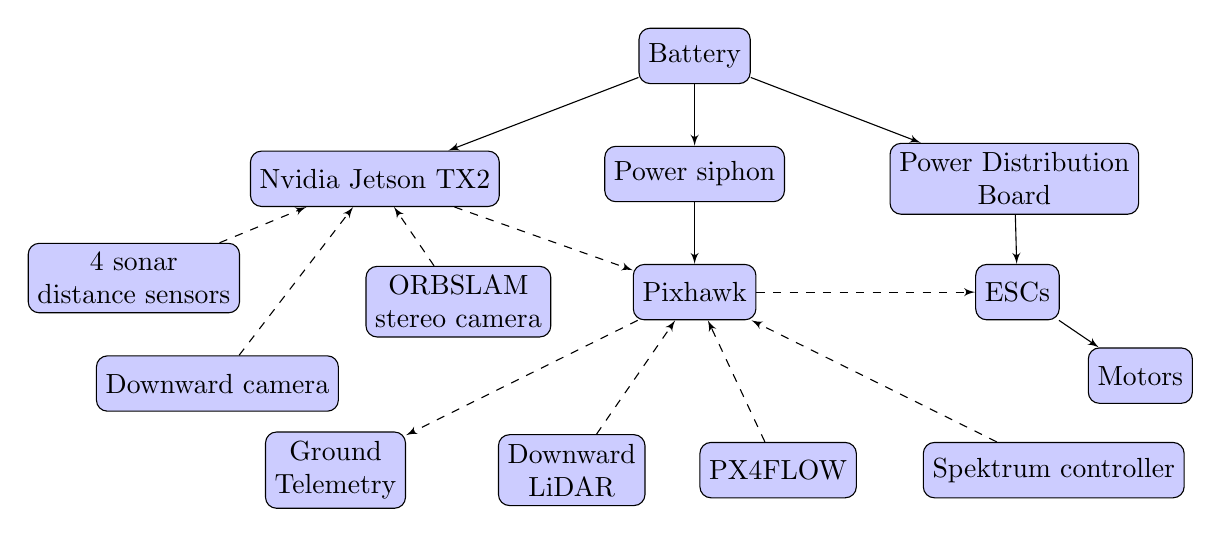
\begin{tikzpicture}[node distance = 1.5cm and 8cm, auto]
				\node [block] (battery) {Battery};
				\node [block, below of=battery] (siphon) {Power siphon};
				\node [block, below of=siphon] (Pixhawk) {Pixhawk};
				\node [block, below right of=battery, xshift=3cm, yshift=-.5cm, align=center] (PDB) {Power Distribution \\ Board};
				\node [block, below left of=battery, xshift=-3cm, yshift=-.5cm] (Jetson) {Nvidia Jetson TX2};
				\node [block, right of=Pixhawk, xshift=2.6cm] (ESCs) {ESCs};
				\node [block, below right of=ESCs, xshift=.5cm] (Motors) {Motors};
				\node [block, below right of=Jetson, yshift=-.5cm, align=center] (StereoCamera) {ORBSLAM \\ stereo camera};
				\node [block, below of=Jetson, xshift=-2cm, yshift=-1.1cm, align=center] (DownCamera) {Downward camera};
				\node [block, xshift=-2cm, yshift=-.2cm, below left of=Jetson, align=center] (Sonars) {4 sonar \\ distance sensors};
				\node [block, below right of=Pixhawk, yshift=-1.2cm] (Flow) {PX4FLOW};
				\node [block, below right of=Pixhawk, xshift=3.5cm, yshift=-1.2cm] (Spektrum) {Spektrum controller};
				\node [block, below left of=Pixhawk, xshift=-.5cm, yshift=-1.2cm, align=center] (LiDAR) {Downward \\ LiDAR};
				\node [block, below left of=Pixhawk, xshift=-3.5cm, yshift=-1.2cm, align=center] (Telemetry) {Ground \\ Telemetry};
				% Draw edges
				\path [line] (battery) -- (siphon);
				\path [line] (siphon) -- (Pixhawk);
				\path [line] (battery) -- (PDB);
				\path [line] (PDB) -- (ESCs);
				\path [line] (battery) -- (Jetson);
				\path [line, dashed] (StereoCamera) -- (Jetson);
				\path [line, dashed] (DownCamera) -- (Jetson);
				\path [line, dashed] (Sonars) -- (Jetson);
				\path [line, dashed] (Flow) -- (Pixhawk);
				\path [line, dashed] (Jetson) -- (Pixhawk);
				\path [line, dashed] (LiDAR) -- (Pixhawk);
				\path [line, dashed] (Pixhawk) -- (Telemetry);
				\path [line, dashed] (Spektrum) -- (Pixhawk);
				\path [line, dashed] (Pixhawk) -- (ESCs);
				\path [line] (ESCs) -- (Motors);
			\end{tikzpicture}
		\caption*{Flowchart of quadcopter electronics \\ \scriptsize *Solid arrows indicate power while dashed lines indicate power+data}
		\end{center}
	\end{figure}

	\pagebreak
	\subsection*{Yearly Milestones}

	2019 - Have a working system, with localization and GPS-denied navigation of multiple drones. These drones should work together to solve the QR code and communicate with a person through an Android app that can transmit voice commands to the drones.

	2020 - Finish all aspects of mission through more networking between the quadcopters, tweak the physique of the drone for better flight control and stability, have better communication between drones to know where enemy drones are at all times, add aesthetic design choices, and test for hours in gyms in as many conditions as possible. 


\section*{AIR VEHICLE}
	\subsection*{Propulsion and Lift System}
			The vehicle utilizes an y axis symmetrical quad-rotor system. This H-frame provides a stable quadcopter for a smaller overall package while maintaining plenty of room for electronics. The frame is lifted by four T-Motor MN2212 KV920-V2.0 motors. These motors provide
			------------fix these numbers---------- 1.8 [kg] of thrust per motor at 100\% throttle when paired with a 4-cell battery and 9.5 [in] propellers for total 7.2 [kg] of thrust. This is necessary for our 3.15 [kg] weight to maintain a 2.2 thrust-to-weight ratio, ideal for battery life and flight time.

			The propellers used with the motors are 9.5 [in] long and made of plastic. These T-Motor propellers provide excellent precision, durability, and efficiency. The rotors are placed to counter-rotate for flight stability and to retain a one-to-one ratio of propellers to motors.
	\subsection*{Power Management System}
The quadcopter uses a 10000 [mAh] 4S 10C LiPo battery and a 2000 [mAh] 3S 15C LiPo battery for power. The 10000 [mAh] 4S 10C LiPo is used to power our ESCs and Motors. With 4 T-Motor U3 K700 motors running at close to the ideal 50\% throttle, a 4 Cell battery was necessary to reach the 1800 [grams] of thrust per motor needed for hovering flight. The 2000 [mAh] 3S 15C LiPo will power the flight control board and Jetson compute units.
\begin{center}
	$T_{min} = \frac{\text{Battery power}(AH) * 60}{\text{Total current drawn by motors}}$
\end{center}

Assuming an average throttle of 65\% for maneuvering, we see a 9 A current draw from each motor, and with a 10 Ah battery, that provides us with 16 minutes of flight time with minimal maneuvering and height change. This gives us plenty of headroom for more intense altitude and positioning changes, which will allow us to move more quickly during the competition, a valuable asset with the given time limitation.
\begin{center}
	Max continuous Amp draw ($A$) = Battery capacity ($Ah$) $*$ Discharge rate ($C$)
\end{center}

To save on weight and space, we chose a 10C discharge rate battery, as this is still more than enough to match the maximum continuous current draw of 25 [A] and maximum practical current draw of 19.4 [A] required by the motors. The 10000 [mAh] battery with a 10C discharge rate gives us a maximum continuous current draw of 100 [A], matching the limit of the motors.

The eCalc online tool was used to validate our calculations, and as seen by the generated graph below, there should be no issue reaching above 10 minute flight times at speeds below 15 [mph].

%		\begin{figure}[!htbp]
%			\begin{center}
%				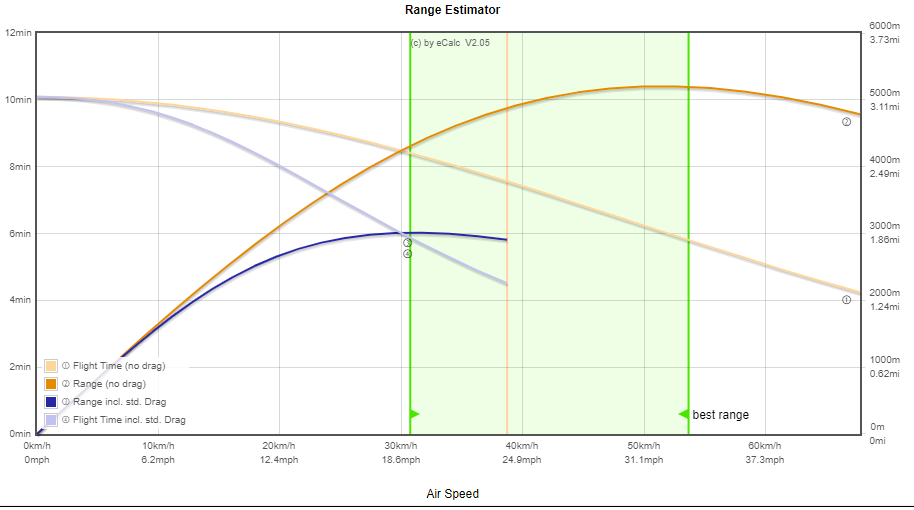
\includegraphics[width=0.75\textwidth]{powerGraph}
%			\end{center}
%		\end{figure}

As for the 2000 [mAh] 3S battery, this battery powers our Pixhawk flight controller and our three Jetson TX2 compute units. This was done partly to dedicate the entirety of the main battery to propulsion to maximize flight time. The other reason is that the speed controllers we chose (T-Motor Air 40A) have no BEC, so a separate battery for the flight controller (and in turn the receiver) was the simplest solution. 2000 [mAh] was chosen because of the slim form factor we were able to find it in, and because it will provide more than adequate power while not adding any significant amount to the quad weight.

	\subsection*{Flight Control System}
		\subsubsection*{Navigation/State Estimation System}
		
			Our system builds off of the robust open source project ArduCopter. ArduCopter, which runs on the Pixhawk, controls the stability of the drone by taking in data from the IMU, compass, altitude ToF, and the optical flow. The ArduCopter flight stack is maintained by hundreds of developers from around the world and the software is deployed on thousands of commercial and recreational drones. The vast community of developers and users ensures refined controls code with lots of features.

			We have made slight modifications to the ArduCopter firmware, which allow us to set the EKF origin. This has been done to make our drones capable of navigating in GPS denied environments. For general waypoint navigation, the drones utilize the ArduCopter EKF that takes in data from the sensors listed above, including the optical flow, compass, and IMU. The EKF position is then queried via mavros so that our controls code can use our position to make intelligent decisions. Additionally, our drones use ORBSLAM running on the Jetson to provide localization data in flight to augment the data from the optical flow sensor while in areas where the ground does not have a textured surface. After those localization and navigation sensors, the controls node also takes in data from the sonar sensors. The controls node determines a waypoint and mode, then does a sanity check on the waypoint before publishing the waypoint until the drone has reached its destination. Over time, the EKF will have some error in comparison to reality. However, using ORBSLAMM, an open-source version of ORBSLAM that contains multimapping, we are able to combat this by correcting the maps through visuals of physical objects (which will not be moving), which is then used to correct the EKF. 
			
		\subsubsection*{Attitude/Position Control System}
		
			Another aspect of navigating in a GPS-denied is concrete information on our position. Using a Teraranger One Time of Flight sensor from Terabee, our drones are able to know their exact altitude. This sensor was chosen due to its extremely light weight over other LiDAR options. This communicates over I2C directly to the Pixhawk where ArduCopter uses that information in the EKF. 
			
			The position control aspect is handled through ORBSLAM running on the Jetson which is then fed into ArduCopter on the Pixhawk. The stereo camera in the front of the aircraft allows visual and depth information of the objects on the field and is used for our position. Additionally, ORBSLAM can potentially fail to get accurate tracking of objects if the drone translates too quickly. This is augmented through the optical flow sensor, which, while not as useful on the non-textured surface should at least ensure that the drone does not lose control. 

			The quadcopter uses eight sensors for flight control. The main sensors used for the navigation of the quadcopter include a downward-facing 1D LiDAR module, a PX4FLOW optical sensor, and the built-in sensors of the Pixhawk 2 flight control board.

			The 1D LiDAR module used is a Time of Flight (ToF) sensor named the Teraranger One. This one-dimensional sensor is directed downward and provides data to determine altitude. The PX4FLOW sensor measures velocity by comparing frame by frame images and measuring the distance traveled and direction. The Pixhawk 2 contains three 3-axis accelerometers, three 3-axis gyroscopes, and two 3-axis compasses. The data from these sensors is used by the Pixhawk onboard system for flight control and maneuvering of the quadcopter.

%		\begin{figure}[!htbp]
%			\begin{center}
%				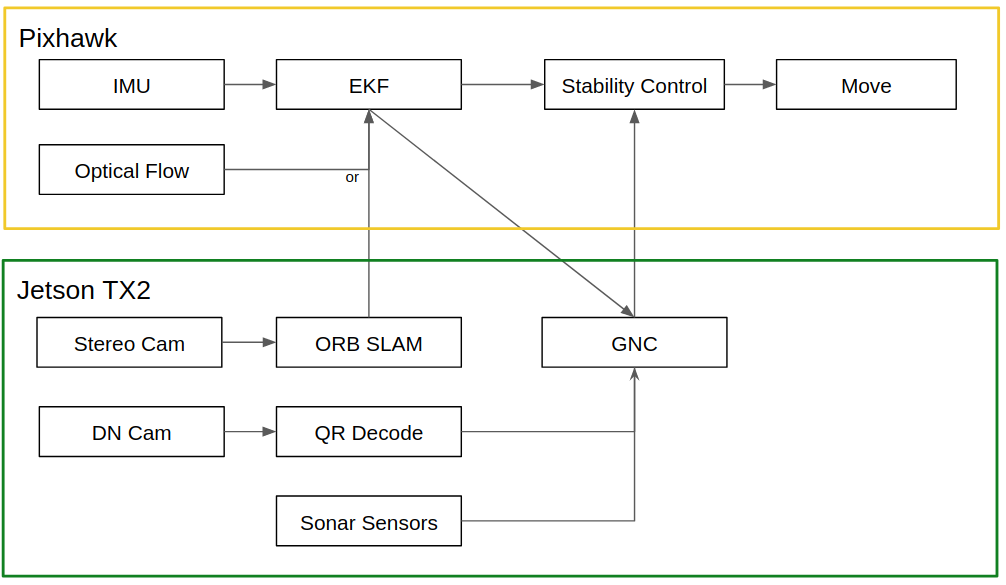
\includegraphics[width=0.75\textwidth]{system}
%				\caption*{Overview of control system}
%			\end{center}
%		\end{figure}

		\subsubsection*{Flight Termination System}
			We will be using ArduCopter's EmergencyStop to act as our killswitch. In the event of catastrophic failure, the safety operator can send the kill signal, and all power will immediately be cut from the drone's ESCs, and in turn, the motors.


\section*{MISSION PACKAGE}
	The drone has been designed to carry all the necessary GNC sensors, an array of sonar sensors, a stereo camera, a downward camera, and a Nvidia Jetson TX2. In addition, the drone carries a telemetry radio, WiFi antennas, and an RC receiver in order to carry out safe flight.
	\subsection*{Perception System}
		\subsubsection*{Target Identification and Behavior}
			For target identification and behavior, the drones fly to defined waypoints where the quadrants of the QR codes are located. Computer vision begins to process the quadrant that is in view. Through our algorithm that uses the inherent features of QR codes, the drone is able to narrow down 
			
			
			For target identification, the drone carries four Logitech C270 USB webcams and one Logitech C210 USB webcam. One of the cameras is located at the bottom of the drone and faces straight downward. The other four cameras are mounted on the bottom side of each arm facing outward. All five cameras are mounted for identifying as many target Roombas surrounding the drone as possible in order to send their coordinates to the strategy node.
			
			There are two main objectives that need to be completed to successfully relay target information to the strategy node. The first objective is to take in the raw video data and detect the target Roombas so that pixel numbers of the centroids of the Roombas in the frame can be sent as output. The second objective is to take the pixel numbers of the centroids of the detected Roombas as input, and then output x and y coordinates relative to the drone using a coordinate transformation and the known height and orientation of the camera with respect to the floor.
			
			In order to accomplish the first objective, an open source software package developed by Joseph Redmon called YOLO (You Only Look Once) is used. More specifically, the TinyYolo version of YOLO was elected to be used since it is lighter and can obtain higher framerates. YOLO is a neural network that can identify user-defined objects once it has been trained. After training the neural network by feeding in approximate 2000 photos of the target Roombas (with the Roombas identified manually), YOLO can reliably identify target Roombas in real time.

		\subsubsection*{Threat Identification and Behavior}
			Our avoidance system takes data from a 2D LiDAR that is used to identify the obstacle Roombas. This data is passed and the strategy node uses this data to weigh possible movements negatively based on their relative position to the obstacle Roombas. The controls node also will use the data, such as in the event an obstacle robot is within 1.5 [m], in which case controls node will issue a waypoint opposite of the minimum vector.

			For completion of Mission 8, the drone must be able to detect the QR code and avoid obstacles, both moving and non-moving. The quadcopter is equipped with a single downward facing camera for reading the quadrant of the QR code. A stereo camera is used for ORBSLAMM for localization. There is also an array of sonar sensors for obstacle avoidance.

			The singular bottom camera is a ELP webcam. This webcam is used for reading the QR code quadrant. The stereo camera in front is also an ELP camera. These cameras were chosen for their very light weight while still allowing adjustment of exposure and other parameters to better read a QR code on an iPad. 
			The array of sonar sensors contains 4 MAXBOTICS 7m I2C sonars. These allow the drone to detect objects on the sides the quadcopter intends to move in. We chose to use this for obstacle detection rather than a 2D LiDAR or webcams to save on weight, space, and computing power. Sonar sensors are very tried and true. Additionally, we opted for sonar rather than radar as radar has a harder time picking up smaller objects, like a drone. 
			
		\subsubsection*{Gesture Identification and Behavior}
			Android app, PocketSphinx. 

	\subsection*{Communications Systems}
		On the Jetsons, data is passed between software nodes via ROS. Data in between our multiple Jetsons is passed via ROS messages through direct ethernet connections. Commands to the flight computer are passed via serial connection with data encoded in MAVLINK messages.
		
		Networking between drones handled through WiFi 2.4 GHz. 


	\subsection*{Man/Machine Interface}
		The drone has a DX7 RC controller interface for system checks and emergency situations. In addition, the flight controller can be monitored via a telemetry radio using Mission Planner. Our autonomous scripts must be initiated by an SSH connection to our Nvidia Jetsons.

\section*{OPERATIONS}
	\subsection*{Flight Preparations}
		\subsubsection*{Checklist}
			\begin{my_enumerate}
				\item Check battery voltage (12.0-12.6V) and insert
				\item Make sure LiDAR, PX4FLOW, and cameras are not covered
				\item Make sure that the props are on in the correct direction (leading edge in)
				\item Make sure prop guards are secure
				\item Make sure Kill Switch is in correct position
				\item Power on controllers
				\item Make sure ground station has good telemetry
				\item Verify critical sensors are giving good data
				\item Plug in TELEM2
				\item SSH start/verify autonomous scripts are running
				\item Make sure everyone is clear of drone
				\item Verify mode switch in Stabilize
				\item Hold safety button
				\item Mode switch to Autonomous
			\end{my_enumerate}

\section*{RISK REDUCTION}
	\subsection*{Vehicle Design}
		\subsubsection*{EMI/RFI Solutions}
		The Arducopter flight stack helps keep interference risk down through the EMI calibration on the Pixhawk. The calibration calculates the magnetic interference correction by formulating a function of the magnetic interference based on the power setting of the motors.

		\subsubsection*{Shock/Vibration Isolation}
		The modern Pixhawk flight controller contains internal damping from the vibration of the drone's structure. The team decided that there is no need for extra damping. After completion of our first drone last year, flight logs from the Pixhawk confirmed that vibration on the built quadcopter was well within recommended amounts. The team believes there is no need to have landing shocks, as the sophisticated Arducopter flight stack has logic to recognize landing. Because of this, nominal landings will not interfere with the guidance or navigation of the drone.


	\subsection*{Safety}
		We took significant steps to ensure safe operation of the quadcopter. In order to keep the quadcopter from flying where we do not want, we have a Spektrum receiver module onboard so our designated pilot can manually control the vehicle. Additionally, we are able to check the status of the quadcopter through our telemetry to our ground station. The structure of the drone is also outfitted with prop guards to mitigate damage to people or property in the event of catastrophic failure. Our prop guards took multiple iterations. We wanted a design that would not interfere with the prop wash, but still be able to prevent damage to the quadcopter itself in the unfortunate event of a collision. The first iteration looked nice, but interfered with the prop wash too much and weighed too much, reducing the thrust. However, the next iteration cut weight and did not interfere with the prop wash.


	\subsection*{Modeling and Simulation}

		To safely test our software throughout the development process, the team implemented a simulation using the Gazebo application. Using this tool, TAR was able to deploy full-scale software in the loop simulation without jeopardizing hardware with each design iteration.

		To employ the Gazebo framework, the team imported a standard quadcopter model from the ArduCopter standard library and Roomba models from Gazebo model library, which were then updated with the color-coded plates and obstacle tubes prescribed for the competition. Additionally, the ground plane within the reproduction was changed to match the texture expected at the competition.

		Gazebo was chosen because of its compatibility with ROS and Ardupilot, the internal communication protocol employed onboard our drone. With this congruence, the exact same software run onboard the drone could be run within the simulation, complete with sensor feedback detected within the simulated instance. C++ scripts could then be utilized to enforce the correct Roomba behaviors, scripting the robots using the same messaging environment as the quadcopter itself (ROS).

		Overall, modeling our software behavior within a Gazebo simulation greatly expedited the development process. By standardizing the simulation setup, tests could be conducted on multiple computers at any time, instead of requiring the sluggish process of updating, calibrating, and flying the physical drone. Additionally, simulation protected the hardware from the accidents and unintentional flight behavior inherent to prototype software.


	\subsection*{Physical Testing}
		Simulation, however, can only prove so much. Eventually, refined software was tested on a model testbed or on the drone itself. Much of the computer vision and general software integration was developed on this testbed, where performance could be verified with the same sensors and computational hardware as the aircraft before full-scale deployment. Even strategy nodes could be tested on this platform, with waypoint predictions vetted before being deployed to the aircraft.

		Flight tests, expectedly, require a specific setting. Generally, Texas Aerial Robotics tested on the roof of the Aerospace building on campus at The University of Texas at Austin. This controlled environment bore witness to hardware implementation throughout our design process, from original flight readiness to early autonomy.

		However, summer development saw additional test flights conducted in a vacant parking garage, but both locations suffered from magnetic inconsistencies which interfered with compass calibrations. Because of this, later tests, including the qualifying run submitted, were conducted in a parking lot to the north of the university.

		Regardless of the setting, each flight test was conducted with constant apparatus: a four meter by four meter test mat printed with the pattern expected at competition to allow optical flow for navigation. Across this mat drives a test Roomba, which accurately recreates both the physical appearance and behaviors of those robots that will be tracked at the venue, complete with top plate and switch. Finally, there is the drone itself, which starts on a corner of the mat, takes off autonomously, and then executes the maneuver to be tested.


\section*{CONCLUSION}
	Texas Aerial Robotics' solutions to the challenges provided by IARC Mission 7 are bountiful and diverse. The physical design process, from the ground up, optimizes flight time while enabling the physical contact required for success. Unique software utilizes input from an expansive collection of sensors to overcome the telemetry limitations imparted by the contest and track the dynamic objectives as they move about the area. Safe operation of these vast networks of interlocking components has been ensured through particular hardware selection and thorough vetting.
	\nocite{redmon2016yolo9000}
	\nocite{GitHubSPACEROBOTICS}
	\nocite{HoughTransform}
	\nocite{CannyEdgeDetection}
	\bibliography{bibliography}
	\bibliographystyle{plain}

\end{document}
